
\documentclass{beamer}

\usepackage{hyperref}
\usepackage{tabulary}
\usepackage{multirow}
\usepackage{booktabs}
\usepackage{subcaption}

\usetheme{metropolis}

\title{Guide for \texttt{thesisdtetiugm} Class File}
\subtitle{Figures in LaTeX}

\author{Muhammad Yasirroni}
\institute{Universitas Gadjah Mada}
\date{\today}

\begin{document}

\begin{frame}
  \titlepage
\end{frame}

\begin{frame}[fragile]
    \frametitle{Example Single Figure}

\begin{verbatim}
\begin{figure}[t]
  \centering
  \includegraphics[width=0.25\textwidth]%
    {../main/images/sample-fig.png}
  \caption{Figure 1 example.}
  \label{fig:fig1}
  % NOTE: the ../ means go up folder
\end{figure}
\end{verbatim}

\end{frame}

\begin{frame}[fragile]
    \frametitle{Example Single Figure}

    Refferencing \ref{fig:fig1} using \verb|\ref{fig:fig1}|

    \begin{figure}[t]
      \centering
      \includegraphics[width=0.25\textwidth]%
        {../main/images/sample-fig.png}  % .. means go up folder
      \caption{Figure 1 example.}
      \label{fig:fig1}
    \end{figure}

\end{frame}

\begin{frame}[fragile]
    \frametitle{Example Multiple Figure}

\begin{verbatim}
\begin{figure}[t]
  \centering
  \subfloat[]{
          \includegraphics[width=0.25\textwidth]%
            {../main/images/sample-fig.png}
          \label{fig:fig2a}}
  \hspace*{-1.2em}  % to setting space between figures
  \subfloat[]{
          \includegraphics[width=0.25\textwidth]%
            {../main/images/sample-fig.png}
          \label{fig:fig2b}}
  \caption{(a) Figure 2a and (b) Figure 2b example.}
  \label{fig:fig2}
\end{figure}
\end{verbatim}

\end{frame}

\begin{frame}[fragile]
  \frametitle{Example Multiple Figure}

  Refferencing \ref{fig:fig2}, \ref{fig:fig2a}, \ref{fig:fig2b} using \verb|\ref{fig:fig2}, \ref{fig:fig2a}, \ref{fig:fig2b}|

\begin{figure}[t]
  \centering
  \subfloat[]{
          \includegraphics[width=0.25\textwidth]%
            {../main/images/sample-fig.png}  % .. means go up folder
          \label{fig:fig2a}}
      \hspace*{-1.2em}  % this is for giving horizontal space for fig 1 and fig 2.
  \subfloat[]{
          \includegraphics[width=0.25\textwidth]%
            {../main/images/sample-fig.png}  % .. means go up folder
          \label{fig:fig2b}}
  \caption{(a) Figure 2a example and (b) Figure 2b example.}
  \label{fig:fig2}
\end{figure}

\end{frame}

% \begin{frame}[fragile]
%     \frametitle{Calling Figure}
  
%     \textbf{Using} \verb|\includegraphics|
  
%     \begin{block}{}
%       \vspace{-2em}
%       \small
%       \begin{verbatim}
% 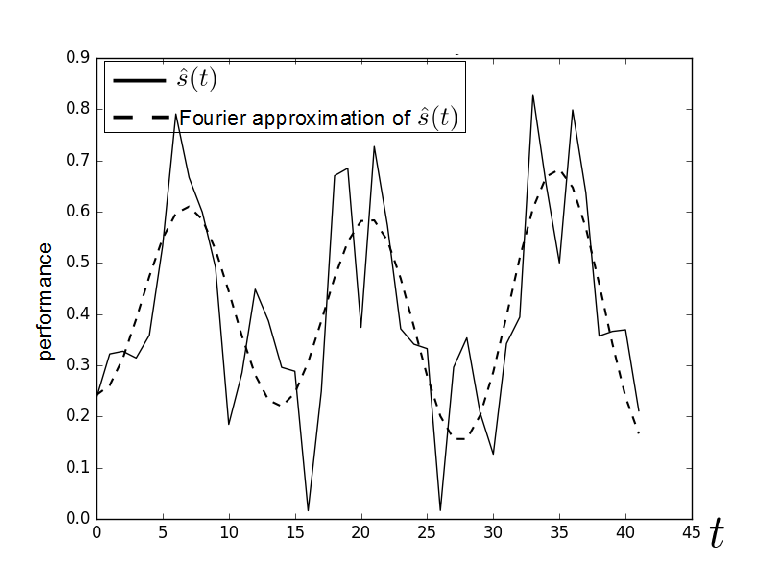
\includegraphics[width=10cm]{images/sample-fig.png}
%       \end{verbatim}
%     \end{block}
  
%     \textbf{Setting} \verb|\includegraphics|
  
%     \begin{itemize}
%       \item \verb|<width=WIDTHcm>| (optional): adjust the width of the image 
%       \item \verb|<FILE_NAME>.ext|: the extension supports various type such as \texttt{.png}, \texttt{.jpg}, and even \texttt{.pdf}. 
%     \end{itemize}
  
%     It is more recommended to not using both \texttt{<height>} and \texttt{<scale>} parameters. Stick with known \texttt{<width>} or page area for the images and let the document decides the height. Alternatively, not using any parameter is also possible to let LaTeX decides the resize.
  
%   \end{frame}

\end{document}
